\documentclass[tikz]{standalone}%

\usepackage[utf8]{inputenx}%  http://ctan.org/pkg/inputenx
% Euler for math | Palatino for rm | Helvetica for ss | Courier for tt
\renewcommand{\rmdefault}{ppl}% rm
\linespread{1.05}% Palatino needs more leading
\usepackage[scaled]{helvet}% ss //  http://ctan.org/pkg/helvet
\usepackage{courier}% tt // http://ctan.org/pkg/courier
\usepackage{eulervm}  %  http://ctan.org/pkg/eulervm
% a better implementation of the euler package (not in gwTeX)
\normalfont%
\usepackage[T1]{fontenc}%  http://ctan.org/pkg/fontenc
\usepackage{textcomp}%  http://ctan.org/pkg/textcomp

\begin{document}
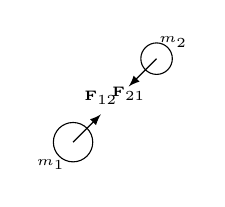
\begin{tikzpicture}
  \draw (0, 0) coordinate (O) circle[radius = .25cm] node[font = \tiny] at
  (225: .4cm) {$m_1$};
  \draw[-latex] (O) -- (45:.5cm) node[pos = 1, above, font = \tiny]
  {$\mathbf{F}_{12}$};
  \draw (45:1.5cm) coordinate (P1) circle[radius = .2cm] node[font = \tiny] at
  ++(45:.3cm) {$m_2$};
  \draw[-latex] (P1) -- ++(225:.5cm) node[pos = 1, below, font = \tiny,
  inner sep = .02]
 {$\mathbf{F}_{21}$};
\end{tikzpicture}
\end{document}
%%% Local Variables:
%%% mode: latex
%%% TeX-master: t
%%% End:
